\section{Transportlaget}
Transportlaget ligger i denne protokolsuite mellem applikationslaget og datalinklaget. Grunden til dette er at netværkslaget ikke er relevant i forhold til node-til-node kommunikation. Transportlaget står for at implementere flow-og fejlkontrol der sørger for at garantere en pålidelig forbindelse mellem to enheder. Transportlaget står derfor for en pålidelig dataoverførsel over de ellers upålidelige underliggende lag.

\subsection{Protokoltype}
Den simpleste protokoltype at implementere er en protokol, hvor data sendes med det samme det modtages fra applikationslaget. Og data sendes op til applikationslaget i det øjeblik transportlaget har modtaget det. Denne protokoltype har hverken fejl- eller flowkontrol. Hvis en pakke går tabt undervejs i forsendelsen f.eks. fordi den er blevet fundet korrupt nede på datalinklaget. Så vil dette aldrig blive opdaget af hverken det modtagende eller det afsendende transportlag. Data vil derfor være gået tabt. For at modvirke dette, kan der implementeres ACK beskeder, der sendes tilbage fra modtageren til afsenderen, og essentielt kvitterer for den modtagende pakke. ACK kan enten sendes tilbage for hver datapakke der bliver modtaget, eller der kan køres kumulative ACK's, hvor et ACK kvitterer for flere pakker ad gangen. Der er blevet valgt at implementere stop-and-wait protokollen, der venter med at sende en ny datapakke, til der er modtaget et ACK for den foregående datapakke. Begrundelsen for dette er, at denne protokol giver mulighed en let-programmérbar fejlkontrol. Implementeringen danner grundlag for at kunne opgraderes til en anden protokol, hvis behovet opstår. Figur \ref{StopAndWait} viser stop-and-wait protokollen.
\begin{figure}[h]
\centering
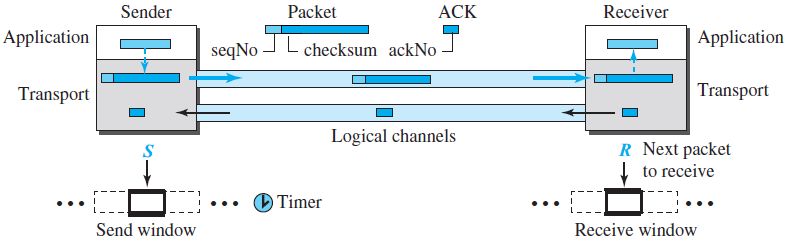
\includegraphics[scale=0.75]{Billeder/StopAndWait.png}
\caption{Stop-and-wait protokollen \\ (modificeret udgave af: Data Communications and Networking, figur 23.20)
\label{StopAndWait}}
\end{figure}

\subsubsection{Effektivitet}
Effektiviteten af en stop-and-wait protokol er meget lav, hvis båndbredden på kanalen er høj og udbredelsestiden er meget lang i kanalen. Hvis der kan sendes mange bits igennem kanalen, og det tager lang tid for dem at nå modtageren, er stop-and-wait ikke det optimale valg. I denne implementering kan stop-and-wait dog godt betale sig, da båndbredden kun er på 160bps og udbredelsestiden er lydens hastighed. Dette medvirker at mediet vil virke instantant, og der derfor ikke ville kunne stoppes ekstra bit ind på mediet, mens der ventes på ACK.

\subsection{Flow-kontrol}
Transportlaget implementerer flow-kontrol i form af de ACK-beskeder, der sendes efter hver data pakke er modtaget. Fordi implementeringen er en stop-and-wait protokol, skal der ventes på ACK inden det næste data kan sendes. Data kan således kun ankomme i rigtig rækkefølge, da en afsender ikke afsender den næste datapakke uden at have modtaget en kvittering. Flowet kan også styres ved ikke at sende et ACK tilbage på en modtaget pakke, hvis modtageren er for optaget til at pakken kan modtages. Således vil afsenderen gentage afsendelsen af pakken efter en timer udløber og modtageren kan så fortsætte med at nægte modtagelse indtil denne er klar.

\subsection{Fejlkontrol}
Der er implementeret fejlkontrol i form af sekvensnumre. Afsenderen af data ved hvilket sekvensnummer den forventer at få tilbage på et ACK, og modtageren ved hvilket sekvensnummer den næste modtagne pakke burde have. Et eksempel på, hvordan fejlkontrollen fungerer kan ses i figur \ref{StopAndWaitFlow}.

\begin{figure}[h]
\centering
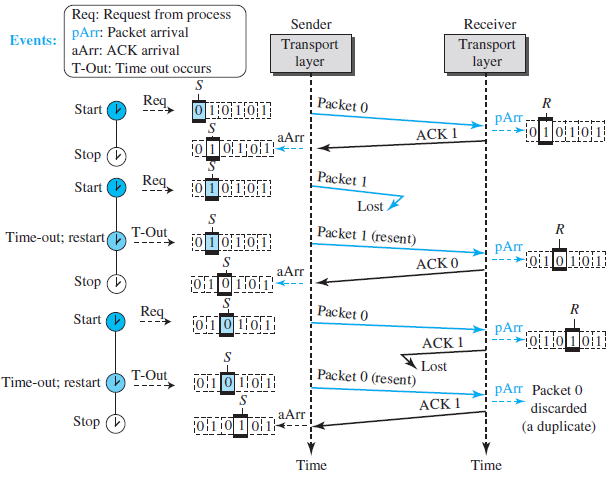
\includegraphics[scale=0.75]{Billeder/StopAndWaitFlow.png}
\caption{Flowdiagram over stop-and-wait protokollen \\(Data Communications and Networking, figur 23.22)
\label{StopAndWaitFlow}}
\end{figure}

\subsection{Implementering}
Transportlaget er implementeret i en klasse uden nogen hjælpeklasser. Afsender-og modtagerdelen kører i samme tråd, og der skiftes mellem at tjekke for modtagen data, og om der skal afsendes noget data. Hele implementeringen kører i en separat tråd fra det ovenliggende applikationslag og opholder derved ikke applikationslaget. Da transportlaget kører i sin egen tråd, er der sørget for at låse delte attributter, når de tilgås. Således opstår der ikke problemer med andre tråde. Hovedfunktionen, der står for at holde transportlaget kørende, er \textit{loop}. Denne startes i en tråd af transportlagets egen constructor.

\subsubsection{Afsending}
Når der afsendes data fra transportlaget, så er transportlaget inde i funktionen \textit{sendData}. Her oprettes der en frame ud fra den nuværende payload, der ligger klar fra applikationslaget. Denne frame afsendes og funktionen \textit{receiveACK} køres. Inde i funktionen checkes der for, om der modtages det korrekte ACK tilbage. Der kører samtidig en timer, som ved udløb resulterer i at transportlaget retransmitterer dataen. Hver gang timeren udløber, inkrementeres der en værdi, og når denne værdi er over grænsen for retransmissionsforsøg(der er fastsat i \textit{constants.h}), så stopper transportlaget med at forsøge at sende datapakken afsted, og venter i et tilfældigt stykke tid(med en nedre grænse på 0 og en øvre grænse fastsat i \textit{constants.h}), før den forsøger at sende igen.

\subsubsection{Modtagelse}
Når der modtages data, så er transportlaget inde i funktionen \textit{receiveData}. Her checkes der for om der ligger en modtaget frame klar i bufferen fra datalinklaget. Hvis dette er tilfældet, checkes der for, hvorvidt dette er en dataframe. Hvis ikke det er en dataframe, smides framen væk. Men hvis det er en dataframe kontrolleres der, om framen har samme sekvensnummer som forventet. Hvis ikke framen har det, så smides den væk og ellers så sendes der et ACK tilbage, og framen smides i et modtagelsesbuffer som applikationslaget kan tilgå.